\documentclass{article}
\usepackage{blindtext}
\usepackage[utf8]{inputenc}

\usepackage{amsthm, amsmath, amssymb}
\usepackage{geometry, setspace, graphicx, enumerate}
\usepackage{listings}
\usepackage[usenames, dvipsnames]{color}
\usepackage{booktabs}

\DeclareMathOperator*{\argmax}{arg\,max}
\DeclareMathOperator*{\argmin}{arg\,min}

\newenvironment{answer}{\par\color{ForestGreen}}{\par}
\setlength\parindent{0pt}

\title{Midterm}
\author{Guoxin SUI}
\date{\today}

\begin{document}
\maketitle
\section{Problem 1}
\begin{answer}
  Assume that the total size of the cake is 1. Denote the physical size of the pieces by $x_1, x_2, x_3$. Since $x_1 + x_2 + x_3 = 1 $and all $x_i \geq 0$, the solution space S is just a triangle. Assign the three people as A,B,C, then we can a traingle where each elementary triangle is an ABC triangle, the A, B, C present the "ownership" of the vertice. A similar triangulation of finer mesh can also be labelled in this way.

  \begin{figure}[h]
   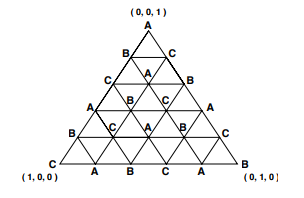
\includegraphics[scale=0.6]{triangle}
\end{figure}

We obtain a new auxiliary labelling of the triangulation by 1’s, 2’s, and 3’s by
doing the following: since each point in the triangle corresponds to a set of cuts of
cake, go to each vertex, and ask the owner of that vertex, “Which piece would you
choose if the cake were cut with this cut-set?” Label that vertex by the number
of the piece that is desired.

Since no one would ever choose an empty piece, each side of $S$ is missing one label corresponding to the piece
that is empty. Hence the Sperner labelling condition is satisfied.

By Sperner’s lemma, there must be a (1, 2, 3)-elementary simplex in the triangulation.
This means that we have found 3 very similar cut-sets in which different people choose different
pieces of cake.

Carry out this procedure for a sequence of finer and finer triangulations,
each time yielding smaller and smaller (1, 2, 3)-triangles. By compactness of the
triangle and decreasing size of the triangles, there must be a convergent subsequence
of triangles converging to a single point. Such a point corresponds to a
cut-set in which the players are satisfied with different pieces.


\end{answer}
\section{Problem 2}
\begin{answer}
    Initiate LH Algorithm:

    $$A = \begin{pmatrix}
          3 & 2 \\
          1 & 3
        \end{pmatrix},
    B = \begin{pmatrix}
          1 & 5 \\
          4 & 2
        \end{pmatrix},$$
\begin{table}[!htb]
  \begin{answer}
\begin{minipage}[t]{.5\textwidth}
\centering
    \begin{tabular}[t]{cccccc}
      \toprule
      P & x1 & x2 & t3 & t4 & = \\
      \midrule
      3 & 1 & 4 & 1 & 0 & 1 \\
      \hline
      4 & 5 & 2 & 0 & 1 & 1 \\
      \bottomrule
    \end{tabular}
\end{minipage}
\begin{minipage}[t]{0.5\textwidth}
\centering
    \begin{tabular}[t]{llllll}
      \toprule
      Q & r1 & r2 & y3 & y4 & = \\
      \midrule
      1 & 1 & 0 & 3 & 2 & 1 \\
      \hline
      2 & 0 & 1 & 1 & 3 & 1 \\
      \bottomrule
    \end{tabular}
\end{minipage}
\end{answer}
\end{table}
$$L(x)=\left\{1,2\right\}, L(y)=\left\{3,4\right\}$$

Second step:

\begin{table}[!htb]
\begin{answer}
\begin{minipage}[t]{.5\textwidth}
\centering
\begin{tabular}[t]{cccccc}
  \toprule
  P & x1 & x2 & t3 & t4 & = \\
  \midrule
  3 & 1 & 4 & 1 & 0 & 1 \\
  \hline
  4 & 9 & 0 & -1 & 2 & 1 \\
  \bottomrule
\end{tabular}
\end{minipage}
\begin{minipage}[t]{0.5\textwidth}
\centering
\begin{tabular}[t]{llllll}
  \toprule
  Q & r1 & r2 & y3 & y4 & = \\
  \midrule
  1 & 1 & 0 & 3 & 2 & 1 \\
  \hline
  2 & 0 & 1 & 1 & 3 & 1 \\
  \bottomrule
\end{tabular}
\end{minipage}
\end{answer}
\end{table}
$$L(x)=\left\{1,3\right\}, L(y)=\left\{3,4\right\}$$

Third step:

\begin{table}[!htb]
\begin{answer}
\begin{minipage}[t]{.5\textwidth}
\centering
\begin{tabular}[t]{cccccc}
  \toprule
  P & x1 & x2 & t3 & t4 & = \\
  \midrule
  3 & 1 & 4 & 1 & 0 & 1 \\
  \hline
  4 & 9 & 0 & -1 & 2 & 1 \\
  \bottomrule
\end{tabular}
\end{minipage}
\begin{minipage}[t]{0.5\textwidth}
\centering
\begin{tabular}[t]{llllll}
  \toprule
  Q & r1 & r2 & y3 & y4 & = \\
  \midrule
  1 & 1 & 0 & 3 & 2 & 1 \\
  \hline
  2 & -1 & 3 & 0 & 7 & 2 \\
  \bottomrule
\end{tabular}
\end{minipage}
\end{answer}
\end{table}
$$L(x)=\left\{1,3\right\}, L(y)=\left\{1,4\right\}$$

Fourth step:

\begin{table}[!htb]
\begin{answer}
\begin{minipage}[t]{.5\textwidth}
\centering
\begin{tabular}[t]{cccccc}
  \toprule
  P & x1 & x2 & t3 & t4 & = \\
  \midrule
  3 & 0 & 18 & 5 & -1 & 4 \\
  \hline
  4 & 9 & 0 & -1 & 2 & 1 \\
  \bottomrule
\end{tabular}
\end{minipage}
\begin{minipage}[t]{0.5\textwidth}
\centering
\begin{tabular}[t]{llllll}
  \toprule
  Q & r1 & r2 & y3 & y4 & = \\
  \midrule
  1 & 1 & 0 & 3 & 2 & 1 \\
  \hline
  2 & -1 & 3 & 0 & 7 & 2 \\
  \bottomrule
\end{tabular}
\end{minipage}
\end{answer}
\end{table}
$$L(x)=\left\{3,4\right\}, L(y)=\left\{1,4\right\}$$

Fifth step:

\begin{table}[!htb]
\begin{answer}
\begin{minipage}[t]{.5\textwidth}
\centering
\begin{tabular}[t]{cccccc}
  \toprule
  P & x1 & x2 & t3 & t4 & = \\
  \midrule
  3 & 0 & 18 & 5 & -1 & 4 \\
  \hline
  4 & 9 & 0 & -1 & 2 & 1 \\
  \bottomrule
\end{tabular}
\end{minipage}
\begin{minipage}[t]{0.5\textwidth}
\centering
\begin{tabular}[t]{llllll}
  \toprule
  Q & r1 & r2 & y3 & y4 & = \\
  \midrule
  1 & 3 & -2 & 7 & 0 & 1 \\
  \hline
  2 & -1 & 3 & 0 & 7 & 2 \\
  \bottomrule
\end{tabular}
\end{minipage}
\end{answer}
\end{table}
$$L(x)=\left\{3,4\right\}, L(y)=\left\{1,2\right\}$$

So we have a mixed strategy equilibrium.
\end{answer}
\section{Problem 3}
\begin{answer}
  \paragraph{(a)}
  \begin{itemize}
    \item Budget constraint :

    $px^i \leq pw^i $
    \item Individual optimality :

    $x^{i*} \in argmax \{u_i(x^i) : px^i \leq pw^{iT},x^i \geq 0 \}$,
    where
    $u^1 = \begin{bmatrix} 3, 0, 0, 0, 0 \end{bmatrix}^T$
    $u^2 = \begin{bmatrix} 0, 4, 2, 0, 0 \end{bmatrix}^T$
    $u^3 = \begin{bmatrix} 0, 2, 1, 0, 0 \end{bmatrix}^T$

    \item Market clearance:

    $\sum_{i\in M} x^i \leq \sum_{i\in M} w^{iT}$
  \end{itemize}

  To get the maximum utility, the agent will put his money on the good where he get most utility with every unit of money since his budget constraints to the equation $px^i \leq pw^i $. So if $x_j^{i*} >0$, that means $\frac{u_j^i}{p_j}$ is the maximum.

  \paragraph{(b)}
  \begin{itemize}
    \item Normalization:
    \begin{itemize}
      \item Everything is owned by someone: Condition fulfilled.
      \item Everything is liked by someone: Elimite the $5_{th}$ good.
      Then we have 4 goods at the market $ N = \begin{Bmatrix} 1,2,3,4 \end{Bmatrix}$.
      The initial endowment of the agents
      $ w^1 = \begin{pmatrix} 0, 2, 0, 1 \end{pmatrix},
      w^2 = \begin{pmatrix} 0, 2, 1, 0 \end{pmatrix},
      w^3 = \begin{pmatrix} 1, 0, 0, 3 \end{pmatrix}$,
      \item Normalization: For the $2_{nd}$ and $4_{th}$ good, divide by total amount.
      The initial endowment of the agents
      $ w^1 = \begin{pmatrix} 0, 1/2, 0, 1/4 \end{pmatrix},
      w^2 = \begin{pmatrix} 0, 1/2, 1, 0 \end{pmatrix},
      w^3 = \begin{pmatrix} 1, 0, 0, 3/4 \end{pmatrix}$,
    \end{itemize}

    \item Atomization:
    \begin{itemize}
      \item Every agent owns one item : replace agent 1, 2, 3 by $ 1_1, 1_2, 2_1, 2_2, 3_1, 3_2$,, then we have
      $6$ markets agents $ M = \begin{Bmatrix} 1_1, 1_2, 2_1, 2_2, 3_1, 3_2 \end{Bmatrix}$,
      where
     $\begin{cases}
        u^{1_1} = \begin{bmatrix} 3, 0, 0, 0\end{bmatrix}^T \\
        u^{1_2} = \begin{bmatrix} 3, 0, 0, 0\end{bmatrix}^T \\
        u^{2_1} = \begin{bmatrix} 0, 4, 2, 0\end{bmatrix}^T \\
        u^{2_2} = \begin{bmatrix} 0, 4, 2, 0\end{bmatrix}^T \\
        u^{3_1} = \begin{bmatrix} 0, 2, 0, 1\end{bmatrix}^T \\
        u^{3_2} = \begin{bmatrix} 0, 2, 0, 1\end{bmatrix}^T
      \end{cases} $

      The initial endowment of the agents
      $\begin{cases}
         w^{1_1} = \begin{pmatrix} 0, 2, 0, 0 \end{pmatrix} \\
         w^{1_2} = \begin{pmatrix} 0, 0, 0, 1 \end{pmatrix} \\
         w^{2_1} = \begin{pmatrix} 0, 2, 0, 0 \end{pmatrix} \\
         w^{2_2} = \begin{pmatrix} 0, 0, 1, 0 \end{pmatrix} \\
         w^{3_1} = \begin{pmatrix} 1, 0, 0, 0 \end{pmatrix} \\
         w^{3_2} = \begin{pmatrix} 0, 0, 0, 3 \end{pmatrix}
       \end{cases} $

      \item Every item is owned by one agent: Rename the same type of items own by different agents and equalize the utilities by an agent on them, then we have
      6 goods at the market $ N = \begin{Bmatrix} 1,2_1, 2_2, 3_1, 3_2, 4 \end{Bmatrix}$.
      $\begin{cases}
         w^{1_1} = \begin{pmatrix} 0, 2, 0, 0, 0, 0 \end{pmatrix} \\
         w^{1_2} = \begin{pmatrix} 0, 0, 0, 0, 1, 0 \end{pmatrix} \\
         w^{2_1} = \begin{pmatrix} 0, 0, 2, 0, 0, 0 \end{pmatrix} \\
         w^{2_2} = \begin{pmatrix} 0, 0, 0, 1, 0, 0 \end{pmatrix} \\
         w^{3_1} = \begin{pmatrix} 1, 0, 0, 0, 0, 0 \end{pmatrix} \\
         w^{3_2} = \begin{pmatrix} 0, 0, 0, 0, 0, 3 \end{pmatrix}
       \end{cases} $
       here
      $\begin{cases}
         u^{1_1} = \begin{bmatrix} 3, 0, 0, 0, 0, 0\end{bmatrix}^T \\
         u^{1_2} = \begin{bmatrix} 3, 0, 0, 0, 0, 0\end{bmatrix}^T \\
         u^{2_1} = \begin{bmatrix} 0, 4, 4, 2, 0, 0\end{bmatrix}^T \\
         u^{2_2} = \begin{bmatrix} 0, 4, 4, 2, 0, 0\end{bmatrix}^T \\
         u^{3_1} = \begin{bmatrix} 0, 2, 2, 0, 1, 1\end{bmatrix}^T \\
         u^{3_2} = \begin{bmatrix} 0, 2, 2, 0, 1, 1\end{bmatrix}^T
       \end{cases} $

      \item Normalization revision: Divide by its size, we get
      $\begin{cases}
         w^{1_1} = \begin{pmatrix} 0, 1, 0, 0, 0, 0 \end{pmatrix} \\
         w^{1_2} = \begin{pmatrix} 0, 0, 0, 0, 1, 0 \end{pmatrix} \\
         w^{2_1} = \begin{pmatrix} 0, 0, 1, 0, 0, 0 \end{pmatrix} \\
         w^{2_2} = \begin{pmatrix} 0, 0, 0, 1, 0, 0 \end{pmatrix} \\
         w^{3_1} = \begin{pmatrix} 1, 0, 0, 0, 0, 0 \end{pmatrix} \\
         w^{3_2} = \begin{pmatrix} 0, 0, 0, 0, 0, 1 \end{pmatrix}
       \end{cases} $
    \end{itemize}


    \item Since everything is liked by someone (The goods that no one likes are eliminated), and an edge from i to j means agent i likes item j, there is non-zero indegree.
  \end{itemize}

  \paragraph{(c)}
  \hfill \break
  In "Linear Utility Market", the goods are initialely distributed to the agents, but they don't have endowment of money.

  In "Fisher Market", there is a seller who owns all the goods, but the agents have endowment of money to buy the goods.


  These differences lead to future differences in market clearance and budget constraints.
\end{answer}

\section{Problem 4}
\begin{answer}
  \begin{itemize}
    \item Bidder 1 get q1 and bidder 2 get q2, \\
    $p_1 = v_2q_1 + v_3q_2 - v_2q_2 = 26$, \\
    $p_2 = v_1q_1 + v_3q_2 - v_1q_1 = 12$
    \item We have
    $\begin{cases}
      u_1(q_1) \geq 0 \\
      u_1(q_1) \geq u_1(q_2) \\
      u_2(q_2) \geq 0 \\
      u_2(q_2) \geq u_2(q_1) \\
      u_3(q_1) \leq 0 \\
      u_3(q_2) \leq 0
    \end{cases}
    \Rightarrow
    \begin{cases}
      v_1q_1 - p_1 \geq 0 \\
      v_1q_1 - p_1 \geq v_1q_2 - p_2 \\
      v_2q_2 - p_2 \geq 0 \\
      v_2q_2 - p_2 \geq v_2q_1 - p_1 \\
      v_3q_1 - p_1 \leq 0 \\
      v_3q_2 - p_2 \leq 0
    \end{cases}
    \Rightarrow
    \begin{cases}
      14 \leq  p_1 \leq 36 \\
      6 \leq  p_2 \leq 14 \\
      14 \leq  p_1 - p_2 \leq 18
    \end{cases}$
    \item Truthful bidding under the GSP protocol is optimal for the buyers since no bidder would change its bid to improve its utility.
    In this case, if all start by bidding their true vale, this is already a Nash equilibrium.
  \end{itemize}
\end{answer}

\end{document}
